\section{Image Classification - MNIST}
\label{sec:Image Classification - MNIST}
Handwritten digit recognition has been a focal point in the field of machine learning and computer vision for several decades. The MNIST dataset, a collection of grayscale images of handwritten digits, has emerged as a canonical benchmark for evaluating various classification algorithms \cite{lecun1998mnist}. In this study, we harness two distinct classification techniques: Convolutional Neural Networks (CNN), which have recently proven to be highly effective for image-related tasks \cite{goodfellow2016deep}, and the traditional k-Nearest Neighbors (k-NN) algorithm, a mainstay in pattern recognition \cite{james2013introduction}. By comparing the performance of these methodologies, we seek to elucidate the strengths and potential limitations inherent to each approach. Our findings contribute to the broader discourse on algorithmic trade-offs between computational complexity, interpretability, and predictive accuracy in the realm of digit recognition tasks.
\subsection{Environment Setup}

The initialization segment of the code sets up the MATLAB environment. To harness the computational power of multi-core processors, a parallel pool is initiated~\cite{matlabparallel}.
\begin{lstlisting}[style=Matlab-editor]
clear all;
close all;
clc;
if isempty(gcp('nocreate'))
    parpool;
end
\end{lstlisting}

\subsection{Data Loading and Preprocessing}

Post-environment setup, the MNIST dataset, which comprises handwritten digits, is loaded. This dataset has extensively been used in the realm of machine learning and computer vision for training and benchmarking~\cite{lecun1998mnist}.
\begin{lstlisting}[style=Matlab-editor]
data = load('mnist.mat');
training_set = data.training;
test_set = data.test;
train_Labels = gpuArray(training_set.labels);
test_Labels = gpuArray(test_set.labels); 
\end{lstlisting}

To streamline the representation for the algorithms, each image is transformed into a vector. Post-transformation, the reshaped data is relayed to the GPU for accelerated computation~\cite{matlabparallel}.
\begin{lstlisting}[style=Matlab-editor]
trainData = gpuArray(reshape(training_set.images, [], size(training_set.images, 3))');
testData = gpuArray(reshape(test_set.images, [], size(test_set.images, 3))');
\end{lstlisting}

\subsection{Image Classification - MNIST: CNN}

The Convolutional Neural Network (CNN) architecture is defined. It comprises Convolution-BatchNorm-ReLU blocks, MaxPooling layers, a fully connected layer, a softmax layer, and a classification layer.

\begin{lstlisting}[style=Matlab-editor]
lgraph = layerGraph([ ... ]);
\end{lstlisting}

\subsection{CNN Architecture Definition}

\begin{lstlisting}[language=Matlab]
%% Define CNN architecture using layerGraph
lgraph = layerGraph([
    imageInputLayer([28 28 1])
    convolution2dLayer(3,8,'Padding','same')
    batchNormalizationLayer
    reluLayer
    
    maxPooling2dLayer(2,'Stride',2)
    
    convolution2dLayer(3,16,'Padding','same')
    batchNormalizationLayer
    reluLayer
    
    maxPooling2dLayer(2,'Stride',2)
    
    fullyConnectedLayer(10)
    softmaxLayer
    classificationLayer]);
\end{lstlisting}

The CNN starts with an input layer designed for images of size \(28 \times 28\) pixels with a single channel (grayscale). This is followed by alternating convolutional layers (with batch normalization and ReLU activation) and max-pooling layers. The CNN concludes with a fully connected layer, a softmax layer, and a classification layer\cite{ciresan2012multi}.
\subsection{Training Configuration}

\begin{lstlisting}[language=Matlab]
options = trainingOptions('adam', ...
    'MaxEpochs', 10, ...
    'InitialLearnRate', 0.001, ...
    'MiniBatchSize', 128, ...
    'ValidationData', {testImages, categorical(testLabels)}, ...
    'ValidationFrequency', 20, ...
    'Verbose', true, ...
    'Plots', 'training-progress', ...
    'ExecutionEnvironment', 'parallel', ...
    'Shuffle', 'every-epoch', ...
    'LearnRateSchedule', 'piecewise', ...
    'LearnRateDropPeriod', 5, ...
    'LearnRateDropFactor', 0.5, ...
    'L2Regularization', 0.0001);
\end{lstlisting}

\subsection{CNN Training and Evaluation}
Training options are set up to use the ADAM optimizer, with various hyperparameters configured such as the number of epochs, learning rate, mini-batch size, and more. Notably, the learning rate is scheduled to decrease every 5 epochs to improve convergence. Validation data is also provided to monitor overfitting.


\begin{lstlisting}[language=Matlab]
%% Train the CNN
[net, info] = trainNetwork(trainImages, categorical(trainLabels),..
lgraph, options);
% Evaluate the trained network
pred = classify(net, testImages);
accuracy = sum(pred == categorical(testLabels)) / numel(testLabels);
fprintf('Test accuracy: %f\n', accuracy);
\end{lstlisting}
\begin{figure}[h]
    \centering
    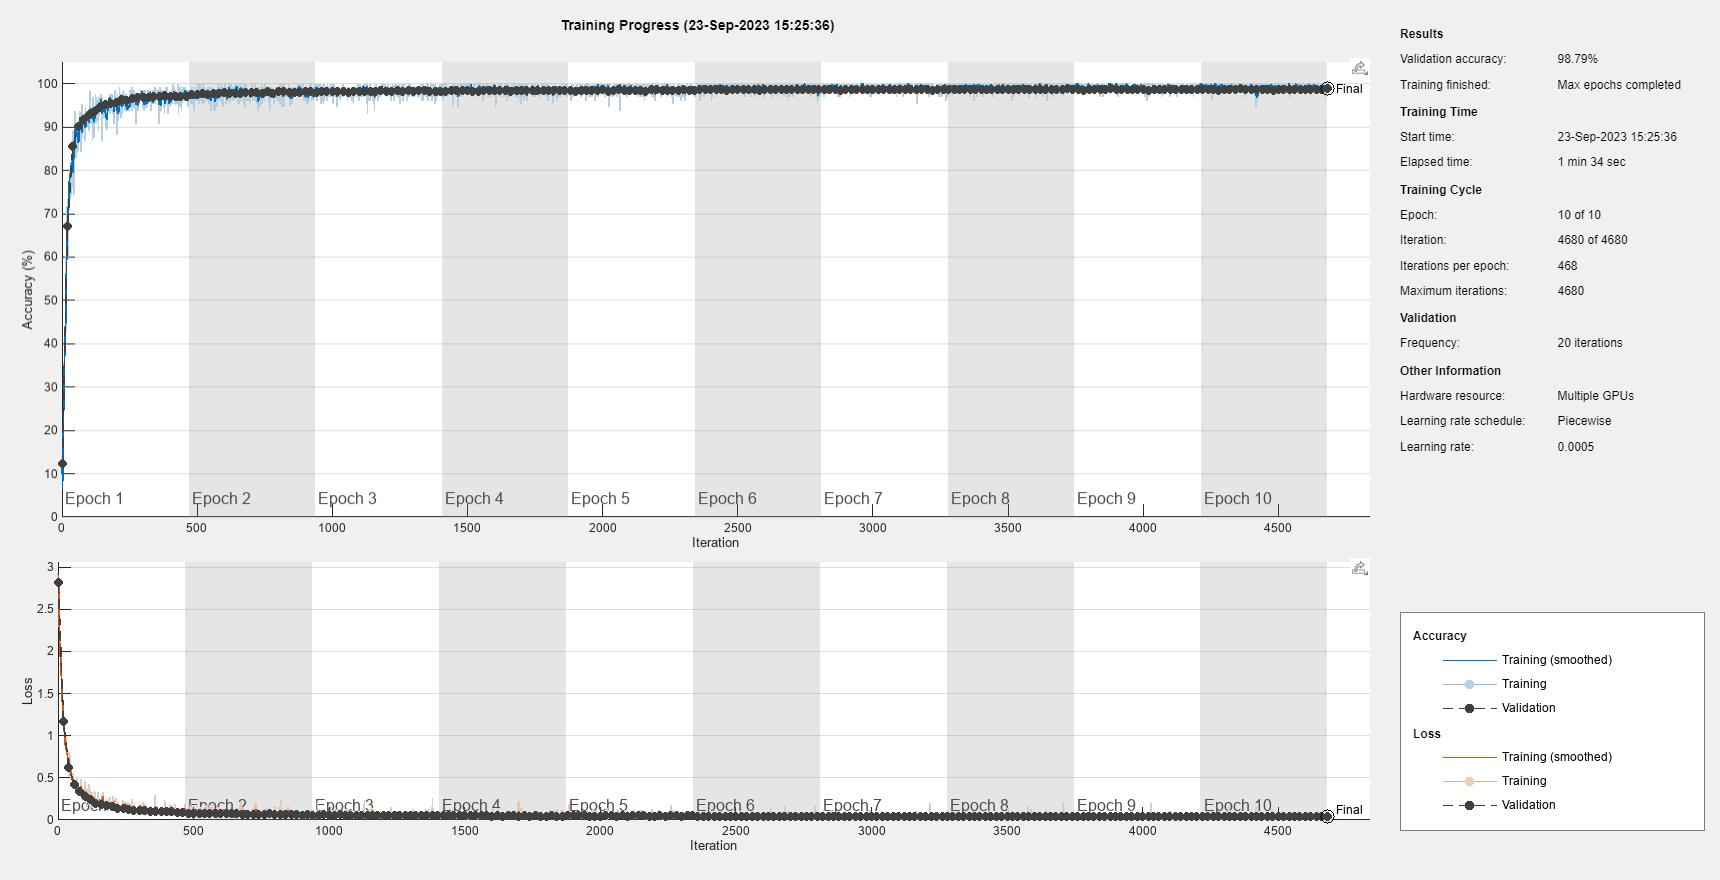
\includegraphics[width=1\textwidth]{cnn_training.jpg}
    \caption{The training progress for each iteration.}
    \label{fig:the training progress} 
\end{figure}

The two plots encompass:
\begin{itemize}
    \item The top-plot depicts the accuracy for each iteration.
    \item The bottom-plot depicts the loss rate for each iteration.
\end{itemize}
\subsection{Image Classification - MNIST: KNN}


The k-Nearest Neighbors (k-NN) algorithm is a non-parametric method that can be employed for classification tasks. The performance of k-NN can be significantly improved when the data's dimensionality is reduced. One such method for dimensionality reduction is Principal Component Analysis (PCA)~\cite{james2013introduction}.



\subsection{Principal Component Analysis (PCA)}

PCA is an essential technique in data science, highlighting variation and capturing dominant patterns in a dataset. Employing PCA can substantially reduce the data's dimensionality without a significant loss of information~\cite{james2013introduction}.

\subsubsection{PCA on Training Data}

The principal components are computed as follows:
\begin{lstlisting}[language=Matlab]
[coeff, score, latent] = pca(gather(trainData));
\end{lstlisting}

\subsubsection{Selecting Principal Components}

To retain 95% of the data's variance, principal components are selected based on the following logic:
\begin{lstlisting}[language=Matlab]
explainedVariance = cumsum(latent) / sum(latent);
numComponents = find(explainedVariance > 0.95, 1);
\end{lstlisting}

\subsubsection{Data Projection}

The training data is projected into the PCA space. The test data is centred using the mean of the training data and then projected:
\begin{lstlisting}[language=Matlab]
trainDataPCA = gpuArray(score(:, 1:numComponents));
meanTrain = mean(trainData, 1);
testDataPCA = gpuArray((gather(testData) - meanTrain)
* coeff(:, 1:numComponents));
\end{lstlisting}

\subsection{Data Visualization}

Visualization provides essential insights. For this dataset, two plots are conceptualized:
\begin{figure}[h]
    \centering
    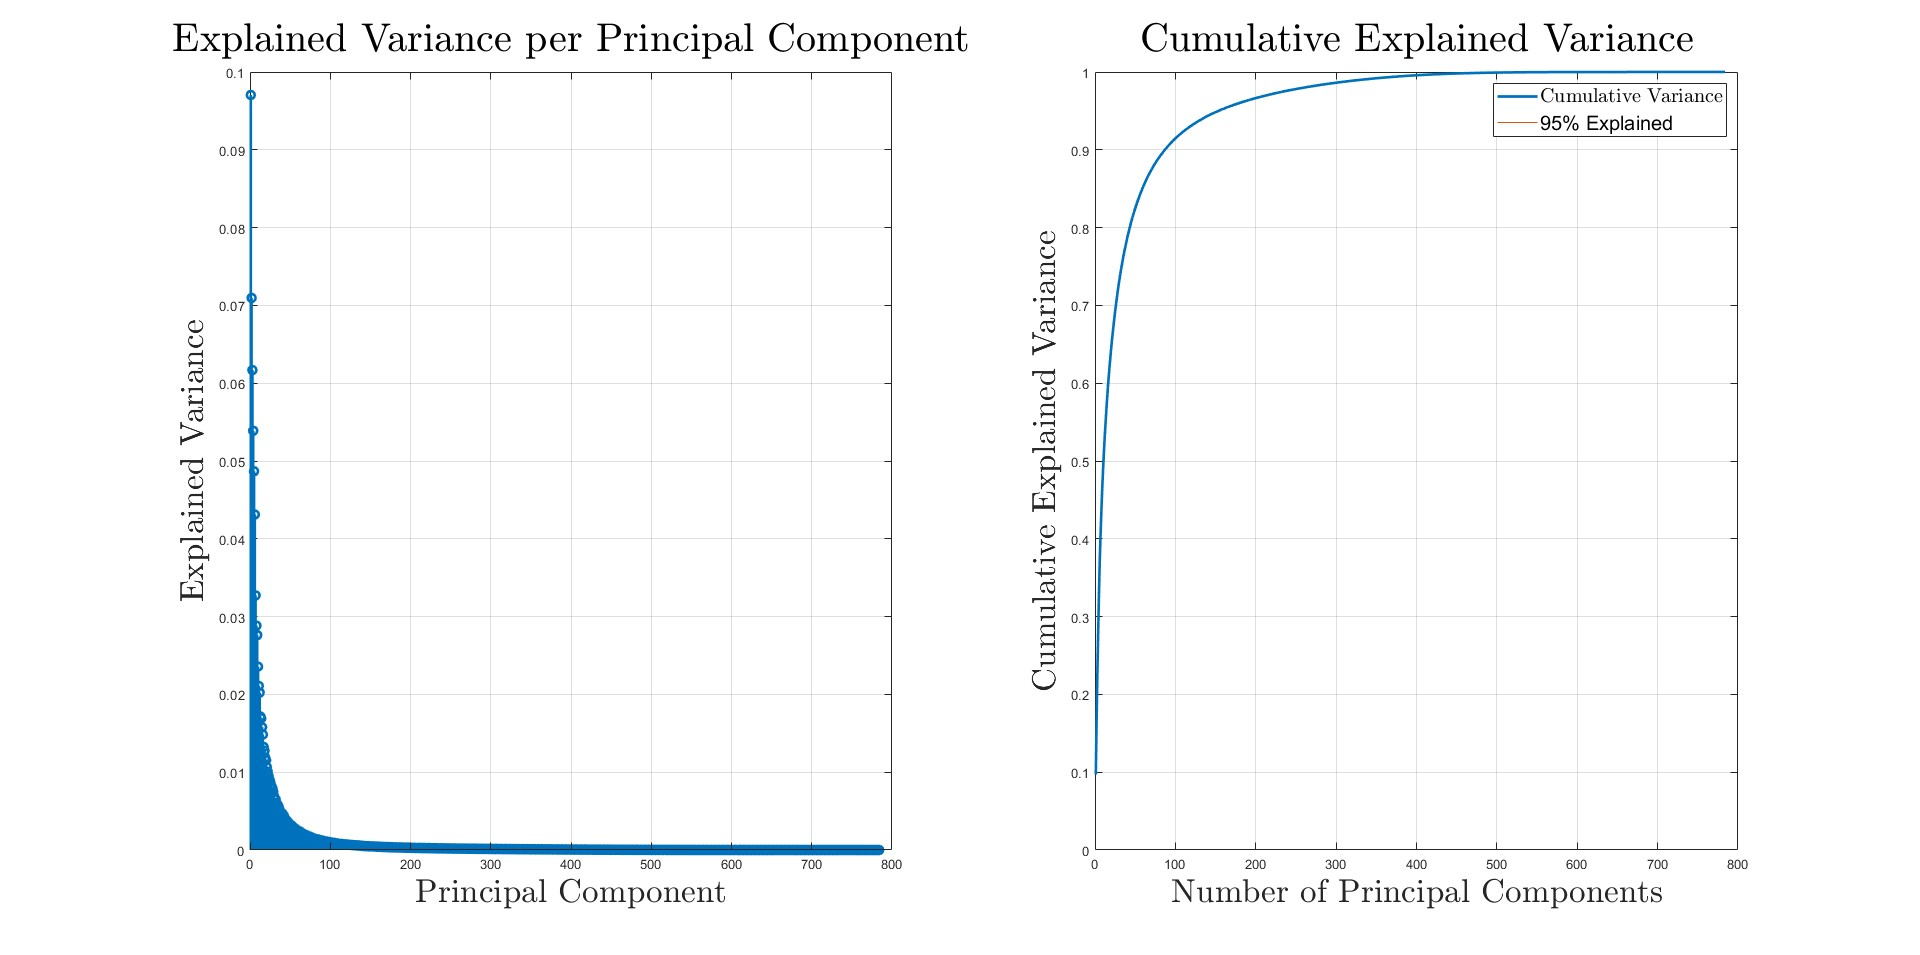
\includegraphics[width=1\textwidth]{PCA_KNN.jpg}
    \caption{Explained Variance Plot.}
    \label{fig:explained_variance} 
\end{figure}

The two plots encompass:
\begin{itemize}
    \item The proportion of variance explained by each principal component.
    \item The cumulative variance explained by the principal components.
\end{itemize}

\subsection{k-Nearest Neighbors Classification}

With the reduced dataset, the k-NN model is trained using the PCA-transformed training data. The choice of `k` (number of neighbors) is set to 5, correlating distance as a metric. After training, the test set predictions are inferred.
\begin{lstlisting}[language=Matlab]

% Train k-NN using the PCA-transformed training data
knn_model = fitcknn(trainDataPCA, train_Labels, 'NumNeighbors', 3, ...
    "Distance","correlation", "DistanceWeight","squaredinverse");
% Predict using the PCA-transformed test data
knn_pred = predict(knn_model, testDataPCA);
\end{lstlisting}
\subsection{Evaluation Metrics}

To understand the model's efficacy, performance evaluation is paramount. A confusion matrix, which juxtaposes actual versus predicted classifications, is analysed. Leveraging this matrix, precision, recall, and the F1-score for each class are computed. These metrics provide an in-depth understanding of the classifier's performance beyond mere accuracy.
\begin{lstlisting}[language=Matlab]

confusionKNN = confusionmat(test_Labels, knn_pred);
.
.
.% Calculate precision, recall, and F1-score
C= confusionKNN;
nClasses = size(C, 1);  % Assuming C is a square matrix
precision = zeros(1, nClasses);
recall = zeros(1, nClasses);
f1Score = zeros(1, nClasses);

for i = 1:nClasses
    TP = C(i, i);
    FP = sum(C(:, i)) - TP;
    FN = sum(C(i, :)) - TP;
    
    precision(i) = TP / (TP + FP);
    recall(i) = TP / (TP + FN);
    f1Score(i) = 2 * (precision(i) * recall(i))...
    / (precision(i) + recall(i));
end
\end{lstlisting}
\subsection{Conclusion}

In our endeavour to classify the MNIST dataset, two different approaches were experimented with: Convolutional Neural Networks (CNN) and k-Nearest Neighbors (k-NN). Each method has its own merits and demerits, and through rigorous evaluation, we gauged their performances.

\subsubsection{Performance Metrics Comparison}

The performance metrics, namely execution time, accuracy, precision, recall, and F1-score, were collected for each method. The comparison between CNN and k-NN using these metrics is provided in Table~\ref{tab:comparison}.

\begin{table}[ht]
    \centering
    \caption{Performance comparison of CNN and k-NN}
    \label{tab:comparison}
    \begin{tabularx}{\linewidth}{l *{5}{>{\centering\arraybackslash}X}}
        \toprule
        Metric & \multicolumn{2}{c}{Value} \\
        \cmidrule(lr){2-3}
         & CNN & k-NN \\
        \midrule
        Execution Time & 94 sec & 2.6 \\
        Accuracy & 98.79\% & 97.23\% \\
        Precision (per class)  & [0.9929 0.9904 0.9864 0.9882 0.9918 0.9833 0.9948 0.9826 0.9847 0.984]\ & [0.9711 0.9716 0.9786 0.9673 0.9714 0.9675 0.9772 0.964 0.9903 0.9649]\ \\
        Recall (per class) & [0.9929 0.9974 0.9855 0.9921 0.9807 0.991 0.9896 0.9864 0.9887 0.9742]
\ & [0.9939 0.9956 0.9748 0.9673 0.9674 0.9686 0.9864 0.965 0.9466 0.9544]\ \\
        F1-score (per class) & [0.9929 0.9939 0.9859 0.9901 0.9862 0.9872 0.9922 0.9845 0.9867 0.9791]
 & [0.9823 0.9835 0.9767 0.9673 0.9694 0.9681 0.9818 0.9645 0.968 0.9596]\ \\
        % Repeat the above three rows for each class
        \bottomrule
    \end{tabularx}
\end{table}

\subsubsection{Confusion Matrix Analysis}

A confusion matrix provides a more detailed breakdown of the classifier's performance by showing the true and false classifications for each class, we can gain further insights into specific areas where each model excels or underperforms.

\begin{figure}[ht]
    \centering
    \begin{minipage}{.5\textwidth}
        \centering
        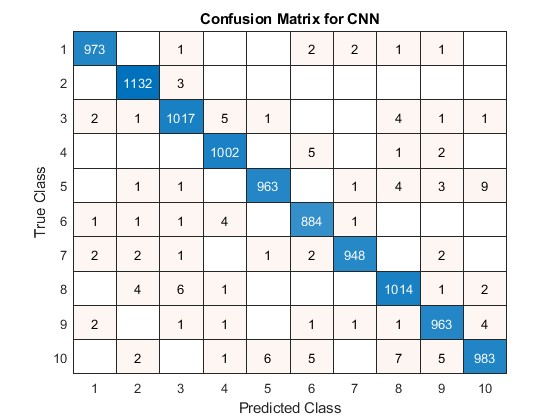
\includegraphics[width=.9\linewidth]{c_mat_cnn.jpg} 
        \captionof{figure}{Confusion matrix for the CNN approach}
        \label{fig:cnn_confusion}
    \end{minipage}%
    \begin{minipage}{.5\textwidth}
        \centering
        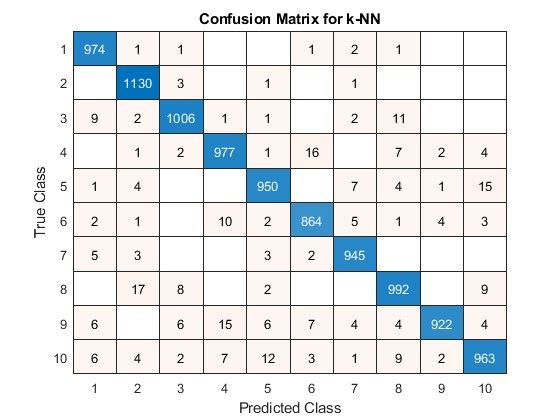
\includegraphics[width=.9\linewidth]{c_mat_knn.jpg} 
        \captionof{figure}{Confusion matrix for the k-NN approach}
        \label{fig:knn_confusion}
    \end{minipage}
\end{figure}

From the confusion matrices presented in Figures~\ref{fig:cnn_confusion} and \ref{fig:knn_confusion}, it is evident that the KNN tends to misclassify class 4 as class 9 more often than the CNN approach.

By scrutinizing the results presented in Table~\ref{tab:comparison} and the confusion matrices, it becomes evident that the CNN method outperforms the k-NN  marginally in terms of accuracy but has a way longer execution time.

.
